\documentclass{article}

%Packages

\usepackage[utf8]{inputenc}

\usepackage[parfill]{parskip}

\usepackage[colorlinks=true,urlcolor=codeblue]{hyperref}

\usepackage{graphicx}

%Document

\title{Software Sustainability - King's workshop exercises}

\author{Martin Chapman}

\date{Friday 2nd May 2025}

\begin{document}

\definecolor{bg}{rgb}{0.95,0.95,0.95}
\definecolor{codeblue}{rgb}{0,0.3,0.6}

\maketitle

\section{Prerequisites}

Please review the \href{https://github.com/martinteaching/sustainability/blob/master/workshops/kcl/2025/README.md}{workshop prerequisites}.

\section{Background}

\begin{center}
    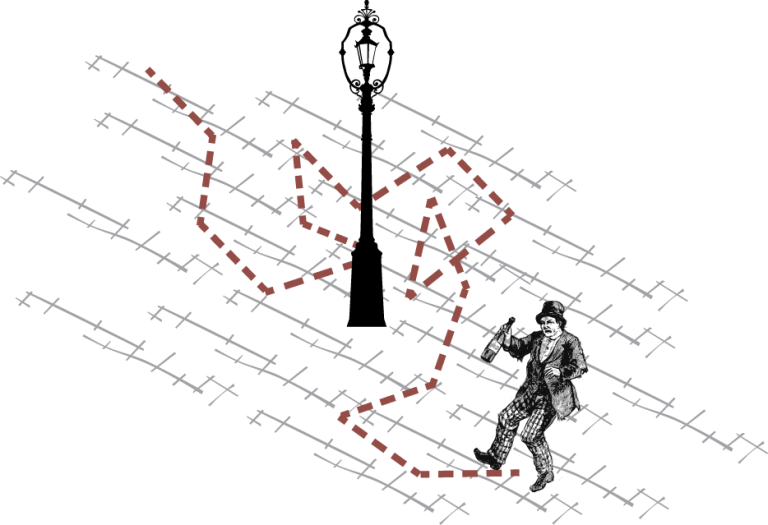
\includegraphics[width=8.6cm]{images/drunkard.png}
\end{center}

Consider the \href{https://en.wikipedia.org/wiki/Random_walk}{Drunkard's walk}: starting at a pub (represented by a point in a 2D space, the dimensions of which are a variable), a drunkard stumbles around (moving either +1 or -1 on the X or Y axis at random) until they reach home (represented by another point in the 2D space).
An example of a drunkard's walk is shown below:

\begin{center}
    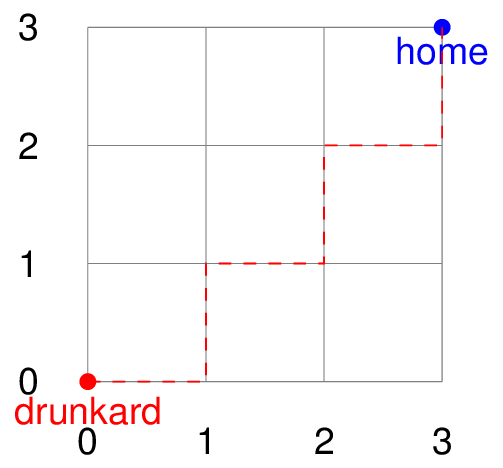
\includegraphics[width=5cm]{images/movement.png}
\end{center}

Here, the drunkard is at position $(0, 0)$. 
Home is at $(3, 3)$. 
The path taken is: $(1, 0)$, $(1, 1)$, $(2, 1)$, $(2, 2)$, $(3, 2)$, $(3, 3)$.

As in the example show, we always assume that the pub is at $(0, 0)$.
Similarly, we always assume that the drunkard's home is at the maximum point ($(3, 3)$, in this example).
If the drunkard reaches the edge of the space (top, right, bottom or left), further travel in that direction is not permitted.

A piece of Python code simulating the drunkard's walk is available \href{https://github.com/martinteaching/sustainability/blob/master/workshops/kcl/2025/resources/drunkard.py}{here}.
It accepts the dimensions of the 2D space as input, simulates the movement of the drunkard towards home, and reports on the path the drunkard took to reach it.
Thus, this code is a piece of research software allowing us to explore the relationship between the size of 2D spaces and the length of a drunkard's walk.

\section{Session 1 (10.10 - 10.50) - Coding practice}

Refactor the current Python code simulating the drunkard's walk so that it adheres to the principles of coding practice discussed in the course.

\emph{You are welcome to reimplement the code using alternative logic first, should you wish to.}

\section{Session 2 (11.00 - 11.50) - Version control}

Make a version of your software, and push it to a remote repository on King's GitHub (\href{https://github.kcl.ac.uk/}{github.kcl.ac.uk}).
Call this repository `drunkard'.

You will need to log in with your k-number and password, if you have not done so before.

\textit{Public Github (\href{https://github.com}{github.com}), should
also work for this task, but should only be used as a backup.}

Additional versions should be made at appropriate points while completing the remaining tasks.

\section{Session 3 (12.00 - 12.50) - Testing}

Write three tests to ensure the following:

\begin{enumerate}

    \item The drunkard eventually reaches home.

    \item Even with a larger grid (10 by 10), the drunkard still eventually reaches home.

    \item The drunkard is \textbf{not} still at position 0, once they leave for home.

\end{enumerate}

Modify your program such that these tests pass, if needed.

You are welcome to add additional tests also.

\section{Session 4 (14.00 - 14.50) - Services}

The supporting materials for this session are available at \newline
\href{https://github.com/martinteaching/sustainability/tree/master/resources}{github.com/martinteaching/sustainability/tree/master/resources}.

Wrap your Python drunkard simulation model in a server and run it.

Move the request for 2D space dimensions to a Javascript client, which, once acquired, sends this information to the server, waits for the drunkard simulation to complete, and then prints the path of the drunkard for the user.

\section{Session 5 (15.00 - 15.50) - Docker}

Dockerise your program -- using a Dockerfile and Docker Compose -- allowing the Python server to run in a container, and the Javascript client to issue requests to it.

\section{Additional Tasks}

If you wish to expand on your solution, create a second Python service that encapsulates the logic required to place $n$ rubbish bins randomly in a 2D space, each with a coordinate. 
Every time your drunkard moves, the simulation code (contained in a service) should call this second service to determine whether the drunkard has hit a bin (i.e. the drunkard's current coordinates are the same as the coordinates of one of the bins).
The total number of collisions should be recorded and reported back to the user along with the drunkard's path.

Under this setup, the client calls a service (drunkard), which in turn calls a second service (bins) as a part of its operation before reporting the results back to the client.

\section{Assessment}

Attendees at the workshop will be given time to review and start these exercises individually, and will then be asked to complete them fully with each other in an online collaborative environment.

Sufficient engagement with these collaborative sessions will result in a `pass' mark for the workshop.

\end{document}
